\documentclass[journal,12pt,twocolumn]{IEEEtran}

\usepackage{enumitem}
\usepackage{amsmath}
\usepackage{amssymb}
\usepackage{graphicx}


\title{Assignment 2 \\ \Large AI1110: Probability and Random Variables \\ \large Indian Institute of Technology Hyderabad}
\author{Ankit Saha \\ \normalsize AI21BTECH11004 \\ \vspace*{20pt} \normalsize  8 April 2022 \\ \vspace*{20pt} \Large ICSE 2019 Grade 12}


\begin{document}
	% The title
	\maketitle
	
	% The question
	\textbf{Question 1(ii)} 
	Solve: $\sin(2\tan^{-1}x) = 1$
	
	% The solution
	\textbf{Solution.}		
	\begin{align}
		\sin(2\tan^{-1}x) = 1
	\end{align}
	
	The general solution to this equation is given by:
	\begin{align}
		2\tan^{-1}x &= (4n + 1)\dfrac{\pi}{2},~n \in \mathbb{Z} \\
		\implies \tan^{-1}x &= (4n + 1)\dfrac{\pi}{4},~n \in \mathbb{Z}
	\end{align}
	
	But we know that the range of $\tan^{-1}x$ is $\left( -\frac{\pi}{2}, \frac{\pi}{2} \right)$
	\begin{align}
		&\implies -\dfrac{\pi}{2} < (4n + 1)\dfrac{\pi}{4} < \dfrac{\pi}{2} \\
		&\implies -2 < 4n + 1 < 2 \\
		&\implies -3 < 4n < 1 \\
		&\implies -\dfrac{3}{4} < n < \dfrac{1}{4}
	\end{align}
			
	As $n \in \mathbb{Z}$, we have $n = 0$
	\begin{align}
		&\implies \tan^{-1}x = \dfrac{\pi}{4} \\
		&\implies \tan(\tan^{-1}x) = \tan\left(\dfrac{\pi}{4}\right) \\ 
		&\implies x = 1
	\end{align}
	$\therefore$ The solution to the equation is $x = 1$
	
	% The graph
	\begin{figure}[!ht]
		\centering
		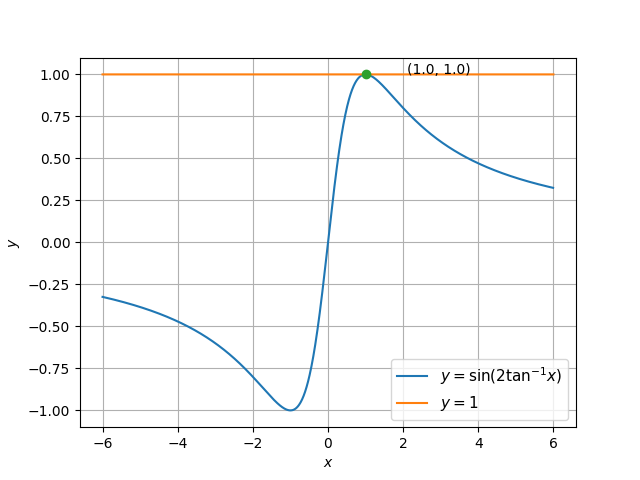
\includegraphics[width=\columnwidth]{figs/fig-1.png}
		\caption{Graph showing the intersection of $y = \sin(2\tan^{-1}x)$ and $y = 1$}
		\label{fig-1}
	\end{figure}
	
\end{document}